\documentclass{article}

% if you need to pass options to natbib, use, e.g.:
%     \PassOptionsToPackage{numbers, compress}{natbib}
% before loading neurips_2020

% ready for submission
% \usepackage{neurips_2020}

% to compile a preprint version, e.g., for submission to arXiv, add add the
% [preprint] option:
%     \usepackage[preprint]{neurips_2020}

% to compile a camera-ready version, add the [final] option, e.g.:
%     \usepackage[final]{neurips_2020}

% to avoid loading the natbib package, add option nonatbib:
\usepackage[final]{neurips_2020}

\usepackage[utf8]{inputenc} % allow utf-8 input
\usepackage[T1]{fontenc}    % use 8-bit T1 fonts
\usepackage{hyperref}       % hyperlinks
\usepackage{url}            % simple URL typesetting
\usepackage{booktabs}       % professional-quality tables
\usepackage{amsfonts}       % blackboard math symbols
\usepackage{nicefrac}       % compact symbols for 1/2, etc.
\usepackage{microtype}      % microtypography
\usepackage{subfig}
\usepackage{caption}
\usepackage{graphicx}
\usepackage{amsmath}
\usepackage{amsthm}
\usepackage{amssymb,amsfonts}
\usepackage{xcolor}
\usepackage{multirow}
\usepackage{soul}
\usepackage{todonotes}
\usepackage{lipsum}


\newcommand{\context}{c}
\newcommand{\expect}{\mathbb{E}}
\newcommand{\expectdiff}{ED}
\newcommand{\scorediff}{\it{SD}}
\newcommand{\latentvariables}{\mathbf{z}}
\newcommand{\inference}{q}
\newcommand{\generation}{p}
\newcommand{\hiddenstate}{\mathbf{h}}
\newcommand{\state}{\mathbf{s}}
\newcommand{\action}{\mathbf{a}}
\newcommand{\reward}{\boldsymbol{r}}
\newcommand{\goal}{g}
\newcommand{\player}{pl}
\newcommand{\pindex}{i}
\newcommand{\prior}{p}
\newcommand{\bin}{\beta}
\newcommand{\boxscore}{b}
\newcommand{\home}{\it{Home}}
\newcommand{\away}{\it{Away}}
\newcommand{\none}{\it{Neither}}
\newcommand{\team}{\it{team}}
\newcommand{\egoal}{\it{goal}}
\newcommand{\Qobs}[2]{Q_{#1}^{\it{obs}}(#2)}
\newcommand{\Qmodel}[3]{\hat{Q}_{#1}(#2,#3)}
\newcommand{\Qbin}[2]{\hat{Q}_{#1}(#2)}
% \newcommand{\observation}{\boldsymbol{x}}
\newcommand{\softmax}{\boldsymbol{\phi}}
\newcommand{\sigmoid}{\boldsymbol{\sigma}}
\newcommand{\observation}{\boldsymbol{o}}
\newcommand{\GaussianParameters}{\boldsymbol{\omega}}
\newcommand{\BernoulliParameters}{\theta}
\newcommand{\system}{VaRLAE\;}
% \newcommand{\system}{VaRLAE}
% for Variational Recurrent Ladder Agent Encoder


% \title{Learning Deep Hockey Player Representations with \\ A Variational Hierarchical Encoder}
%\title{Contextualize In-Game Variations for Team Sports}

\title{Learning Agent Representations for Ice Hockey}

% The \author macro works with any number of authors. There are two commands
% used to separate the names and addresses of multiple authors: \And and \AND.
%
% Using \And between authors leaves it to LaTeX to determine where to break the
% lines. Using \AND forces a line break at that point. So, if LaTeX puts 3 of 4
% authors names on the first line, and the last on the second line, try using
% \AND instead of \And before the third author name.

% \author{%
%   Guiliang Liu\thanks{Corresponding Author: Guiliang Liu}, Oliver Schulte\\
%   School of Computing Science\\ 
%   Simon Fraser University, Burnaby, Canada \\
%   \texttt{gla68@sfu.ca, oschulte@cs.sfu.ca} \\
%   \And
%   Pascal Poupart, Mike Rudd \\
%   Cheriton School of Computer Science \\
%   University of Waterloo, Waterloo, Canada\\
%   \texttt{\{ppoupart,jmrudd\}@uwaterloo.ca} \\
%   \And
%   Mehrsan Javan \\
%   Sportlogiq, Montreal, Canada \\
%   \texttt{mehrsan@sportlogiq.com} \\
% }

\author{Guiliang Liu$^{1}$, Oliver Schulte$^{1,3}$, Pascal Poupart$^{2,4}$, Mike Rudd$^{2,4}$, Mehrsan Javan$^{3}$\\
$^{1}$School of Computing Science, Simon Fraser University\\
$^{2}$Cheriton School of Computer Science, University of Waterloo\\
$^{3}$SLiQ Lab, Sportlogiq\\
$^{4}$Vector Institute \\
\texttt{gla68@sfu.ca, oschulte@cs.sfu.ca}\\
\texttt{\{ppoupart,jmrudd\}@uwaterloo.ca, mehrsan@sportlogiq.com}
}

\begin{document}

\maketitle

\begin{abstract}
  Team sports is a new application domain for agent modeling with high real-world impact. A fundamental challenge for modeling professional players is their large number (over 1K), which includes many bench players with sparse participation in a game season. The diversity and sparsity of player observations make it difficult to extend previous agent representation models to the sports domain. This paper develops a new approach for agent representations, based on a Markov game model, that is tailored towards applications in professional ice hockey. We introduce a novel framework {\it player representation via player generation}, where a variational encoder embeds player information with latent variables. The encoder learns a context-specific shared prior to induce a {\it shrinkage effect} for the posterior player representations, allowing it to share statistical information across players with different participation rates. To capture the complex play dynamics in sequential sports data, we design a Variational Recurrent Ladder Agent Encoder (VaRLAE).  This architecture provides  a contextualized player representation with a hierarchy of latent variables that effectively prevents latent posterior collapse. We validate our player representations in three
  %{\it major} 
  major sports analytics tasks. Our experimental results, based on a large dataset that contains over 4.5M events, show state-of-the-art performance for our VarLAE on facilitating 1) identifying the acting player, 2) estimating expected goals, and 3) predicting the final score difference.
\end{abstract}

\section{Introduction}
% More and larger event stream datasets for sports matches facilitate applying advanced machine learning to model complex sports dynamics.
% Team sports are a strong real-word testbed as the game rules define 
Team sports define complex interactions with a rich action space and a heterogeneous state space~\cite{Gudmundsson17TeamSports}. 
As more and larger event stream datasets for professional sports matches become available, advanced machine learning algorithms have been applied to model the complex dynamics of sports games. These models facilitate many applications with high real-world impact, such as predicting match outcomes~\cite{bunker2019machine}, assessing the performance of players or teams~\cite{Liu2018,decroos2018action,schulte2017markov,Liu2020DeepSoccer}, and recommending tactics to coaches~\cite{schwartz}. 
However, previous models often pool observations of different players without capturing the specific roles and behaviors of each athlete. Neglecting the special characteristics of individual players significantly compromises the  model performance for the application tasks~\cite{ganguly2018problem}.
% Neglecting differences among individual players lose valuable information.

A promising approach to incorporating player information into sports statistics is {\em deep agent representation.}
Learning agent representation in a sports game raises new challenges that require a novel solution 
%and existing agent embedding methods are inadequate to model professional players 
for several reasons: {1)}
Previous methods commonly learn a representation of agents’ {\em policy}~\cite{GroverRepresent18,ChandakAction19, AlbrechtSurvey18,Kormushev13RLRobotics, Arnekvist2019PolicyEmbedding,Chen2019ActionEmbedding}. 
The policy embedding methods model only how a player acts in a {\em given} match context, and thus fail to capture the statistical information about which match contexts players are likely to act in, as well as their immediate outcomes (rewards).
{2)} Although %these 
policy embeddings can facilitate  the construction of an artificial agent in {\it control} problems, 
%human players are resistant to control and 
the goal of agent representation in sports analytics is {\em predicting} game-relevant events using player identity information~\cite{ganguly2018problem,schwartz}.
{3)} Previous agent representation models are often validated in virtual games instead of physical sports. They assume a limited number of agents (usually less than 10) and {\it sufficient} observations for each of them. In contrast, professional sports leagues often have upwards of one-thousand players, and many  bench (backup) players play only a few (less than $20$) games
% have {\it very limited chances of performing} 
in a season.
% (\textcolor{blue}{For players who do not play often, deciding to field them more, or to recruit them from another team is one of the most challenging yet also most consequential decisions for team managers.})
%Deciding whether players who do not play often should be 
The large number of agents and unbalanced observations result in unstable embedding models that overfit to players with high participation during training, which undermines both the training convergence and the predictive performance of underlying policy representations~\cite{AlbrechtSurvey18}.


This work describes a novel player representation framework that learns {\em player representations via player generation.} Conditioning on the current game context, the generation model predicts the distribution of the currently acting player. During this process, we learn a distribution of latent variables as the context-specific prior, allowing a neural encoder to derive an approximate posterior as a {\it contextualized representation} for the observed player. We train the encoder by maximizing an Evidence Lower Bound (ELBo, Equation~(\ref{eq:elbo})) that moves the posterior for each player toward the prior mode. This {\em shrinkage effect}~\cite{kruschke2014doing} is ideal for player representations, because: 1) It allows information to be transferred between the observations of different players and draws closer the representations of players who share 
%many 
statistical similarities.
%under a game context. 
2) A shrinkage estimator prevents the encoder from overfitting to players with high participation, allowing our representation to generalize to the diversity and the sparsity of context-aware player distributions.
%based on the context information.

Following our representation framework, we design a Variational Recurrent Ladder Agent Encoder (VaRLAE) to learn player representations. \system utilizes a ladder structure~\cite{SonderbyLadderVAE16} where, in each layer, latent variables condition on a context variable and the representations from upper layers, based on a causal dependence of latent variables that follows a Markov Game Model~\cite{Littman1994}. To incorporate play history into player representations, \system applies a recurrent network  %model play dynamics in 
to sequential sports data.
The ladder hierarchy of latent variables embeds both context and player information, which effectively improves the generative performance and prevents posterior-collapse~\cite{SonderbyLadderVAE16,HePosteriorCollapse19}.
% (i.e., 
%the $KL$ term in ELBo vanishes to 0.
%and 
% the model generates the player distribution from context variables without using the latent variables). 
% This design allows \system to model the play dynamics in the sequential games data.

We demonstrate the generative performance of our \system on a massive National Hockey League (NHL) dataset containing over 4.5M events. \system achieves a leading identification accuracy (>12\% for the players with sparse participation) over other deterministic encoders and policy representation models. 
% The learned player representations are illustrated to show how well the shrinkage effect facilitates generating contextualized embeddings.
To study how much the learned player representations improve downstream applications, we assess two major tasks in sports analytics: Predicting expected goals and final match score differences. 
Empirical results show the improvement in predictive accuracy after incorporating the embeddings generated by \system as input. 

% \textcolor{blue}{I don't know whether we should talk about the details of comparison method.}
% \textcolor{orange}{
% Comparison baselines include the following. {\em Deterministic Encoders}: We utilize a general deterministic auto-encoder for one-hot player representations that conditions on the current match context. Focusing on sports player embeddings, a recent work~\cite{ganguly2018problem} trained a neural encoder 
% %to embed players.
% % \st{They extracted the middle layer from the trained encoder and used it as a player embedding to facilitate the training of other primary tasks.}
% %They trained the encoder as a deterministic regressor, 
% to map game contexts to the identity of the currently present players. 
% The deterministic models shows large estimation variance, especially when the player presence has a multimodal distribution.
% Experimental results show the predictive improvement due to our A-VRNN encodings over  the deterministic comparison methods.} \todo{quantify how much improvement} 

% \textcolor{orange}{
% Like recent work on applying machine learning to sports analytics, our A-VRNN is based on a Markov game model. We therefore compare with a state-of-the-art agent representation framework from reinforcement learning [cite]. In the RL approaches, agents are identified with their policies i.e. a distribution $\pi(a|s,\it{player}=i)$ that maps states to action probabilities for a given player $i$. Our experiments show that our A-VRNN encodings provide more informative player representations than the state-of-the-art policy representation [give the name]. The fundamental reason for this is that a policy representation fails to capture the statistical information about which match states players are likely to act in. For example in hockey, offensive players are more likely to act in the offensive zone than defensive players. 
% }

% \textcolor{orange}{
% The most common approach to incorporating player information in sports statistics is to use a {\em hierarchical model} \cite{kruschke2014doing,Gelman06}. Existing hierarchical models in sports assume a fixed parametric form (e.g. linear or categorical), and learn different parameter estimates for each player. In a Bayesian hierarchical model, the posterior parameter distribution for each player is shrunk toward the mode of a shared prior. {\em Shrinkage} substantially reduces the estimation of variance~\cite{Murphybook12}, but it is hard to find a suitable distributional form for the complex dynamics of team sports.
% }

% \textcolor{orange}{
% Neural networks are general function approximators well-suited to capturing sports dynamics. To combine the advantages of both hierarchical models and neural approximators, we apply the VRNN model~\cite{ChungKDGCB15}. The VRNN is a special conditional variational auto-encoder (CVAE) that generates observations at a current time step $t$ conditional on a previous history. Our agent A-VRNN model is trained to generate a probability distribution over which player is acting at time $t$, given the previous match history, current context features (e.g. location at time $t$), and the current action $a_t$. We use the VRNN encoding component to compute a {\em contextualized} player representation (see 
% see Figure~\ref{fig:player-represent}). VRNN encoding achieves a shrinkage effect because player representations are regularized towards a common (context-dependent) prior. 
% }

\section{Related Work}
We describe the previous works that are most related to our approach.

{\bf Agent Representation.}
% Learning the representation for an agent involves modelling its tendency to act under different states, and a common approach for embedding the agents information is modeling their policy. For example, p
Previous works~\cite{guenter2007reinforcement,KoberP08policy,Kormushev13RLRobotics} represented an agent by imitating its policy in the learning-from-demonstration~\cite{Argall09lfd} setting.  Some recent works~\cite{AlbrechtSurvey18,GroverRepresent18,RubinPoker11,BakkesHehavior12} extended  behavioral modelling to a multi-agent system. Multi-agent representations include modeling interactions between agents and their opponents' behavior for reasoning about a specific goal, such as winning a poker or video game. These interactive policy representations scale poorly to a large number of agents~\cite{AlbrechtSurvey18,AlbrechtR16}.
% A compromise is partitioning the agents into smaller groups such that there is high expected correlation within groups but only little %or no correlation 
% between groups~\cite{AlbrechtSurvey18,AlbrechtR16},  but this method can not be extended to player representation, because a professional league assigns the equal amount of competition for the players in two teams.}
To identify the agent representations, \cite{GroverRepresent18} introduced a triplet loss that encourages an exponential distance between deterministic embeddings for different agents.
%Previous work have demonstrated the success of 
Policy representations have been successful for the design of artificial agents in control problems, such as games or robot control. However, 
%such techniques can not be directly extended to determine the behavior of 
real human players in professional sports cannot be controlled like artificial agents. For sports analytics,
%the general sports analytic tasks, 
the goal of representing players is {\em predicting} game-relevant events using player identity information~\cite{ganguly2018problem,schwartz}. This goal often requires modeling as many aspects of a players' behavior as possible, so we also represent 
not only the agents' policies, but also 
the distribution of states and rewards associated with them.
Some recent works~\cite{Sadeghian2019SoPhie,Gupta18SocialGan} have proposed modeling the trajectories of multiple agents to predict their future paths. They applied a Generative Adversarial Networks (GAN) to discriminate fake from real trajectories without explicitly learning agent representations, and thus their models are not directly applicable to embed  player identities.

{\bf Variational Encoders.} Variational encoders apply a set of latent variables $\latentvariables$ to embed the observations $\observation$. The latent variables form a disentangled representation where a change in one dimension corresponds to a change in one factor of variation~\cite{BengioRepresentation13}. Such representations are often interpretable~\cite{KimM18,Higgins17BetaVAE} and have been applied to embed information in multiple domains ( e.g. robot skills~\cite{HausmanEmbedSkills18} and task environment~\cite{zintgraf2019variational}).
% , and state-action sequences~\cite{WhitneyACG20}. 
The learned representations can significantly facilitate generating many kinds of complicated data, such as images~\cite{kingma2013auto,WalkerDGH16} and action trajectories~\cite{Zhan19basketballvrnn,Sun19basketballvrnn}. To learn these representations, the Variational Auto-Encoder (VAE) maximizes an Evidence Lower Bound (ELBo): $\log p(\observation) \geq \mathbb{E}_{\inference(\latentvariables|\observation)}\Big[\log\generation(\observation|\latentvariables)\Big] -\mathcal{D}_{\text{KL}}(\inference(\latentvariables|\observation)\| p(\latentvariables))$. The traditional VAE design uses 
a Gaussian encoder and a neural decoder to model the approximate posterior $\inference(\latentvariables|\observation)$ and the likelihood function $\generation(\observation|\latentvariables)$ respectively. 
% Their parameters are optimized to maximize an Evidence Lower Bound (ELBo) $\log p(\observation) \geq \mathcal{D}_{\text{KL}}(\inference(\latentvariables|\observation)\| p(\latentvariables))+\mathbb{E}_{\inference(\latentvariables|\observation)}\Big[\log\generation(\observation|\latentvariables)\Big]$. 
%An extension designed a 
The Conditional VAE (CVAE)~\cite{WalkerDGH16} is an extension that conditions the generation process on some external environment variables. To model sequential data, the Variational Recurrent Neural Network (VRNN)~\cite{ChungKDGCB15}  combines CVAE with LSTM recurrence. 
%To model dependencies among latent variables,  introduces a
The Ladder VAE (LVAE) models dependencies among latent variables with a top-down structure that effectively prevents posterior collapse~\cite{SonderbyLadderVAE16}. 
% The Graph VAE~\cite{He19GVAE} allows learning more flexible dependency structure on a hierarchical of latent variables, but it is difficult to combine its graphical inference structure with conditional variables and recurrent signals.
% Our \system absorbs the advantages from all above models to learn a robust player representation. 

% \paragraph{Hierarchical Models in Sports Analytics.}
% Many previous works~\cite{Gelman06,davis2015simulator}
% % on shrinkage models 
% have built multi-level hierarchical models for capturing player information in sports analytics and estimated the parameters of the posterior with Bayesian inference.
% % Bayesian inference naturally incorporates the shrinkage effect into estimating model parameters. 
% % % The shrinkage effect pulls the estimates of low-level parameters closer together than they would be if there was not a higher-level distribution, and generally, 
% % The shrinkage effect encourages lower-level parameters to shift toward the mode of the higher-level distributions, which can significantly reduce the variance of estimation. 
% % Similar hierarchical models have many applications in sports analytics, 
% For example, a previous work~\cite{kruschke2014doing} built a hierarchical model to estimate the batting abilities for individual baseball players.
% For each batter, they estimate the posterior probability of hitting the ball, from a prior conditioning on player positions.
% Accordingly, for players in the same position, despite the difference in performance, their representations shrink toward the position-specific mode. 
% % leaves the posterior distribution of their difference being nearly zero.
% % Such a shrinkage effect can facilitate our player embedding model. Given the intuition that similar players are likely to appear in similar contexts, 
% Our model achieves a similar shrinkage effect that encourages the posterior of player representation to shift toward the mode of a dynamic context-specific prior. A key difference is that neural networks can approximate general functions, whereas previous work on sports analytics assumed a known fixed functional or distributional form for the hierarchical model.

% \paragraph{Contextualized Embedding.}
% As a promising technique of incorporating background knowledge into representation learning, contextualized embedding has been extensively studied in Natural Language Processing (NLP). For example, A previous work~\cite{AkbikBV18} proposed a contextual string embedding. The embedding model contextualizes words by their surrounding text. Therefore the same word will have different embeddings in different contexts. 
% Another recent work~\cite{PetersNIGCLZ18} used contextualized embeddings to model complex characteristics of word use (e.g., syntax and semantics).
% %, and extended the application of embeddings across different linguistic contexts. 
% They showed that contextualized embeddings can be easily added to existing models and significantly improved the state-of-the-art across six challenging NLP problems. The above embedding models are only applicable under the NLP environment where context and embedding targets are both words. In this work, we extend contextualized embeddings to the environment of professional sports and learn the player representations conditioning on complex game contexts.
% % , we compute contextualized embeddings for NHL players conditioning on the game contexts (including the current observation and play history). 
% % Our results also demonstrate the benefit of applying contextualized embeddings in identifying pids and predicting expected goals. 
% % \textcolor{blue}{explain why we don't we compare with the word embedding model.}

% \begin{figure}%
%     \centering
%     \subfloat[Contextualized Player Representation\label{fig:player-represent}]{{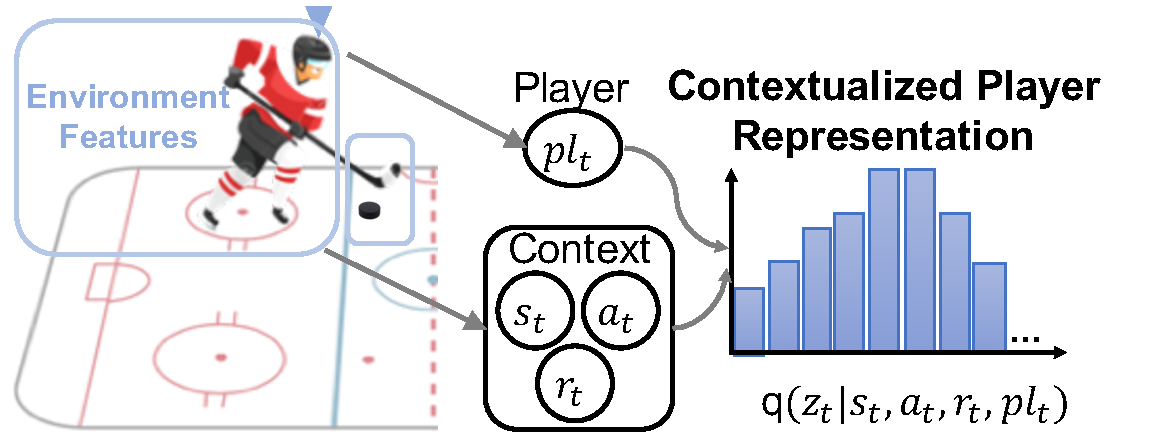
\includegraphics[width=0.5\columnwidth]{./figures/player-embedding-example.pdf}}}%
%     \quad
%     \subfloat[Learning player embedding\label{fig:flow-chart}]{{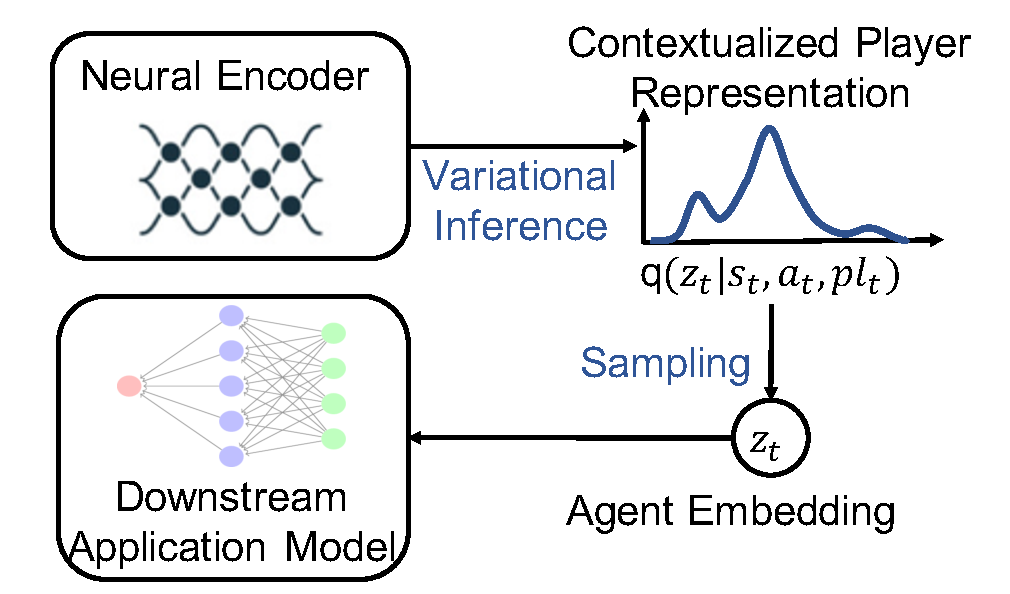
\includegraphics[width=0.3\columnwidth]{./figures/flow-chart.pdf} }}%
%     \caption{(a) The contextualized player representation, where we sample embeddings (latent variables) $\latentvariables_{t}$ for player $\player_{t}$ under game context ($\state_{t},\action_{t}$). $\state_{t}$ contains game history information (see Section~\ref{sec:context-nhl}). (b) System flow for learning contextualized player representations and validating them in the downstream application tasks.
%     } 
% \end{figure}

% % \subsection{Agent Representations in RL?} 


% % \section{Problem Formulation}
% % \textcolor{blue}{Shorten the idea and place it under the introduction.}
% % To utilize the player information, we formulate this task into two sub-problems: 1) How to learn a robust player embedding model and 2) How will the embedding influence the mode performance in solving the practical problem.

% % For the first problem, we investigate the game environment, actions and games statistic that feature a player's overall playing skill.  
% % To include the feature information into our embedding, our model is train to solve a secondary prediction problem: Given the condition a on-the-ball action $\action_{t}$, game context $\state_{t}$ (including locations, game time etc.) and play history $\hiddenstate_{t-1}$, who is likely to be the player   $\player_{t}$ performing the action. In this sense, our model summarizes all the conditional feature information into a embedding vector, and unlike previous works which assigns a deterministic embedding vector to each player, our model learns to generate a comprehensive embedding vector $\latentvariables_{t}$ conditioning on various game or player features. 

% % To answer the second question, we look into two commonly studied problems including 1) game outcome prediction and 2) player performance evaluation. 
% % In the recent years, many works have applied machine learning models to solve those problems, but a common drawback of the proposed models is they considered very limited player information.
% % To overcome the limitation and validate our conditional embedding,
% % % demonstrate the benefit of adding more player information
% % , we input the learned player embedding vectors into their model and check whether and how the embedding will improve the model performances. 

\section{Player Representation Framework}
We introduce the contextual variables for ice hockey and the player representation framework.
\subsection{Contextual Variables for Ice Hockey Players}~\label{sec:context-nhl}
We model the ice-hockey games with a Markov Game Model~\cite{Littman1994}: $G=(\mathcal{S}, \mathcal{A}, \mathcal{T}, \mathcal{R}, \Omega)$. 
At each time step $t$, an agent performs an action $\action_{t} \in \mathcal{A}$ at a game state $\state_{t} \in \mathcal{S}$ after receiving an observation $\observation_{t} \in \Omega$. 
This process generates the reward
$\reward_{t} \sim R(\state_t, \action_t)$ and the next state $\state_{t+1} \sim \mathcal{T}(\state_t, \action_t)$.
% Applying this framework, 
For each game, we consider event data of the form $[(\observation_0,\player_0,\action_0,\reward_0),(\observation_1,\player_1,\action_1,\reward_1),$ $\ldots,(\observation_{t},\player_{t},\action_{t},\reward_{t}),\ldots]$:
at time $t$, after observing %environment  signal 
$\observation_{t}$
% ~\footnote{\textcolor{blue}{We represent it as a feature vector specifying a value of the features listed in Table~appendix at a discrete-time step $t$.} }
, player $\player_{t}$ takes a turn (possesses the puck) and chooses an action $\action_{t}$, which produces a reward $\reward_{t}$ (goal score) .

The play dynamics for the acting player $\player_{t}$ can be captured by the following contextual variables:
1) The {\it game state} $\state_{t}$ describes the game environment where the action is performed. 
To alleviate the partial observability of observations, a game state includes the game history: $\state_{t} \equiv (\observation_t, \reward_{t-1},\action_{t-1},\player_{t-1},\observation_{t-1},\ldots,\observation_{0})$. We utilize the RNN hidden states $\hiddenstate_{t-1}$ to capture the game history~\cite{littlestone}, so $\state_t \equiv (\observation_{t},\hiddenstate_{t-1})$.
2) The {\it action} $\action_t$ records the action of the on-puck player. 3) The {\it reward} $\reward_{t}$ denotes whether a goal is scored after performing $\action_t$. As in general RL, the sequence state-action-reward can be interpreted {\em causally} in sports: the player makes observations summarized in a state signal $\state_t$, which influences his action $\action_t$; together with the environment, the state and action influence whether the player scores a goal. The corresponding causal graph is $\state_{t}\rightarrow \action_{t}\rightarrow\reward_{t}$. 
% \todo[color=red,inline]{there should be an arrow from state to reward I think.}

%
\subsection{Player Representation via Player Generation}~\label{subsec:player-represent-framework}
We introduce our framework of learning player representations through modeling a player generation distribution: $p(\player_{t}|\state_{t},\action_{t},\reward_{t})$. This distribution describes the {\em where and what} of a player's characteristics: what game states they tend to act in, what their actions are, and what immediate outcomes they achieve.
% a player’s tendency to act under different game states and the immediate outcome, which makes it an appropriate target for learning contextualized embedding for each player. 
Inspired by previous work~\cite{HausmanEmbedSkills18,zintgraf2019variational,WhitneyACG20}, we utilize latent variables $\latentvariables_{t}$ as a representation of game context, which can be decoded to the distribution of current acting players:
\begin{align}
    p(\player_{t}|\state_{t},\action_{t},\reward_{t}) & =  \int p(\player_{t}|\latentvariables_{t})p(\latentvariables_{t}|\state_{t},\action_{t},\reward_{t}) \mathrm{d}\latentvariables_{t}
\end{align}
where, {\it before} observing the acting player $\player_{t}$, the {\bf context-aware} prior \space $p(\latentvariables_{t}|\state_{t},\action_{t},\reward_{t})$ models which players are likely to perform $\action_{t}$ under $\state_{t}$ and receive $\reward_{t}$. 
The motivation for a contextualized representation is that the behavior of sophisticated agents, like professional players, is highly sensitive to context and it is difficult to learn a fixed representation that can adequately describe a player's tendencies under every game context.
{\it After} observing the target player $\player_{t}$, we 
% follow the design of Conditional Variational Auto-Encoder (CVAE)~\cite{WalkerDGH16} and
learn an approximate posterior $q(\latentvariables_{t}|\state_{t},\action_{t},\reward_{t},\player_{t})$ as a {\bf contextualized player representation}, so the complete generative process becomes:
\begin{align}
    p(\player_{t}|\state_{t},\action_{t},\reward_{t}) 
    & \approx \int p(\player_{t}|\latentvariables_{t})q(\latentvariables_{t}|\state_{t},\action_{t},\reward_{t},\player_{t}) \mathrm{d}\latentvariables_{t} \label{eq:generation}
\end{align}
During training, our ELBo objective (Equation~\ref{eq:elbo}) induces a {\bf shrinkage effect} through minimizing the Kullback–Leibler (KL) Divergence between the posterior representation for each individual player $q(\latentvariables_{t}|\state_{t},\action_{t},\reward_{t},\player_{t})$ and a context-specific prior $p(\latentvariables_{t}|\state_{t},\action_{t},\reward_{t})$. A shrinkage estimator is ideal for learning player representation for team sports because 1) it has strong statistical properties that allow information to be transferred between the observations of different players, or of the same player in different game contexts. 
The shrinkage effect becomes stronger for players who share many statistical similarities under a game context, which %asymptotically 
draws their representations closer.
This naturally formalizes our intuition that {\em statistically similar players are assigned similar representations under similar game contexts.} 
2) The Shrinkage term also works as a regularizer that prevents the player representations from overfitting to some frequently-present players. Compare to a deterministic auto-encoder, the stochastic shrinkage estimator can generalize to more agents with sparse observations.

In contrast to a policy representation~\cite{GroverRepresent18,WhitneyACG20,ChandakAction19} that captures how a player acts in a {\em given} state, our player representation also models when and where they act, and how successful their actions tend to be. Since our context includes actions, states, and rewards, our learned embeddings reflect how players differ in all three of these dimensions. 
% We refer to this property as the \textbf{context-completeness.} \footnote{\textcolor{red}{Os: this is not used later. Not too keen on this concept.}}


% We utilize a conditional variational auto-encoder whose encoder
% $q(\latentvariables_{t}|\player_{t},\state_{t},\action_{t},\reward_{t}) 
% $
% implements the agent encoder $f$. This approach is motivated by three key benefits. (1) \textbf{ Context-Awareness.} The behavior of sophisticated agents, like professional players, is highly sensitive to context. 
% It is difficult to learn a fixed representation that can adequately describe a player's tendencies under every game context. 
% Conditioning on context provides a 
% % , rather than aiming to learn a single fixed prior representation.
% dynamic contextualized player representation.
% (2) \textbf{Context-Completeness.} Players are characterized not only by how they act, but also by when and where they act, and how successful their actions tend to be. Since our context includes actions, states and rewards, our learned embeddings reflect how players differ in all three of these dimension. In contrast a policy representation captures how a player acts in a {\em given} state but not what states they are likely to act in. (3) \textbf{Shrinkage Effect.} In a hierarchical model, shrinkage moves the posterior distribution for each player toward the prior mode. Shrinkage estimators have strong statistical properties because they allow information to be transferred between the observations of different individuals. 
% The shrinkage effect becomes stronger for players who share many statistical similarities under a game context, which %asymptotically 
% draws their representations closer.
% This naturally formalizes our intuition that {\em statistically similar players are assigned similar representations under similar game context.}
% The VAE incorporates a shrinkage effect in the ELBO loss function ( Equation~\eqref{eq:loss} below) through minimizing the Kullback–Leibler Divergence between the posterior representation for each individual player and a context-specific prior. 
% Our VAE architecture is carefully tailored for our sports application; the next section presents the details. 



% % summarizes the observed player actions, the game environment and the rewards.
% % , with a joint distribution $\generation(\player_{t}, \state_{t}, \action_{t}, \reward_{t})$. 
% This generative distribution can be factored into two components: $p(\player_{t}, \state_{t}, \action_{t}, \reward_{t}) = p(\state_{t},\action_{t}, \reward_{t})\generation(\player_{t}|\state_{t},\action_{t}, \reward_{t})$ where the player-independent component $p(\state_{t},\action_{t}, \reward_{t})$ represents the game context (observed action, state and reward at $t$) and the \textbf{player generation model} 
% \begin{align}
% p(\player_{t}|\state_{t},\action_{t},\reward_{t}) = \int\mathrm{d}\latentvariables_{t}p(\player_{t}|\latentvariables_{t})p(\latentvariables_{t}|\state_{t},\action_{t},\reward_{t}) \label{eq:generation}
% \end{align}
%  models the dependency between the observed game context and the acting player $\player_{t}$.
% \textcolor{blue}{We define a vector with latent variables $\latentvariables_{t}$ to model a game context describing the action $\action_{t}$ performed in game states $\state_{t}$ as well as the immediate outcome $\reward_{t}$. Conditioning on the given context variables, the ideal $\latentvariables_{t}$ can be accurately mapped to the distribution of players that are likely to presence in the game context. Without knowing the acting player, these latent variables constitute a representation for game context $p(\latentvariables_{t}|\state_{t},\action_{t},\reward_{t})$. In this work, we use this context representation as the prior to derive our contextualized player representation $p(\latentvariables_{t}|\state_{t},\action_{t},\reward_{t},\player_{t})$ {\bf after} observing the player $\player_{t}$}.

% \textcolor{blue}{Previous works often learn a $\latentvariables_{t}$ to condition on all context variables. Considering the causal graph of Markov Decision Process (MDP) $\state_{t}\rightarrow \action_{t}\rightarrow\reward_{t}$, we explore the hierarchies of stochastic variables and define a multi-layer dependency structure $\latentvariables_{\state,t}\rightarrow\latentvariables_{\state,t}\rightarrow\latentvariables_{\reward,t}$. At each layer, the latent variables embeds a context variable. The posterior (contextualized player representation) becomes: }

% \begin{align} \label{eq:generate-de-composite}
% \hspace{-0.1in}\generation(\latentvariables_{t}|\state_{t},\action_{t},\reward_{t},\player_{t}) = 
% \int \mathrm{d}\latentvariables_{\state,t}\:\mathrm{d}\latentvariables_{\action,t}\Big[
% p(\latentvariables_{\reward,t}|\reward_{t},\latentvariables_{\action,t},\player_{t})p(\latentvariables_{\action,t}|\action_{t},\latentvariables_{\state,t},\player_{t})p(\latentvariables_{\state,t}|\state_{t},\player_{t})
% \Big]
% \end{align}

% \textcolor{blue}{It describes a player's tendency to act under different game states and the immediate outcome, which makes it {\em an informative target for learning a contextualized embedding for each player.} 
% }

\begin{figure}[!htbp]
    \centering
    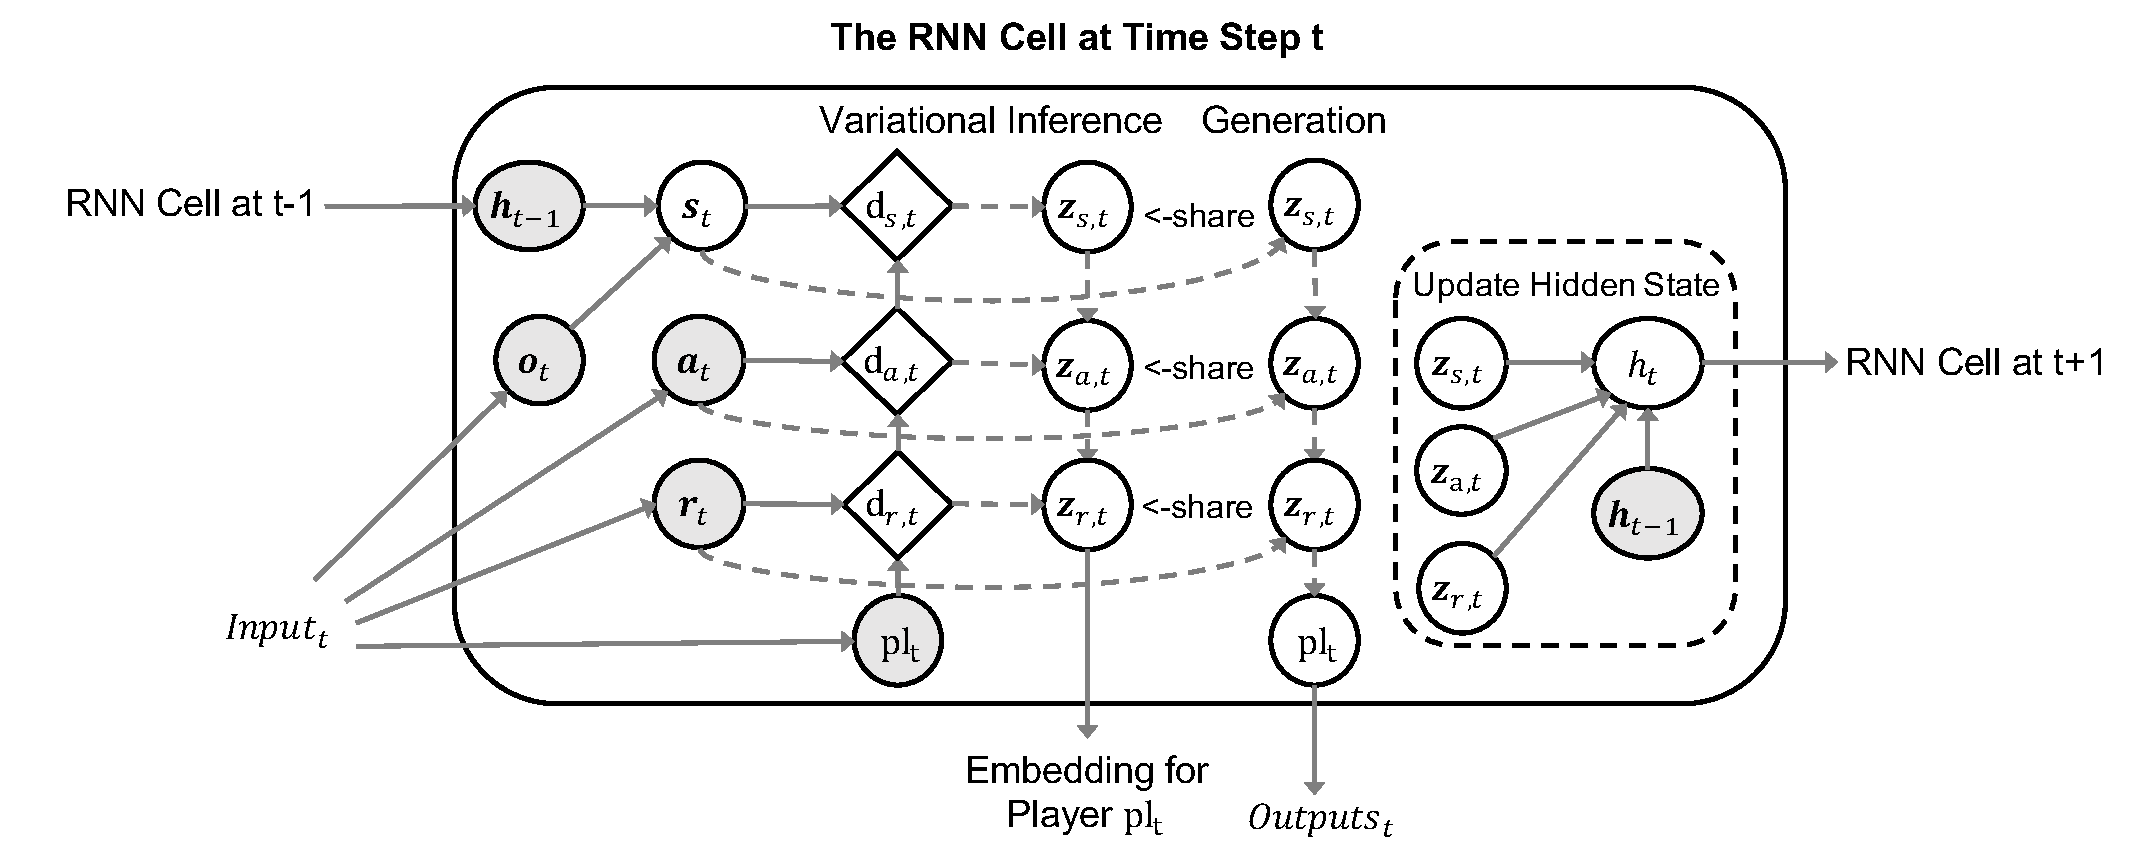
\includegraphics[width=1\columnwidth]{figures/clvrnn-graph.pdf}
    \caption{Our \system model includes a conditional Ladder-VAE at every RNN cell. \system applies a top-down dependency structure
    % $\latentvariables_{\state,t}\rightarrow \latentvariables_{\action,t}\rightarrow \latentvariables_{\reward,t}$
    ordered as the sports causal relationship (Section~\ref{sec:context-nhl}).
    % : $\state_{t}\rightarrow \action_{t}\rightarrow\reward_{t}$.
    The thick/dash lines denote logical-functions /stochastic-dependence. The shaded nodes are given.
    }
    \label{fig:varlae-graphical-model}
\end{figure}

\section{A Variational Agent Encoder for Learning Agent Representations}
%This section introduces our  
Our \system architecture \system (Figure~\ref{fig:varlae-graphical-model}) for learning player representations follows our our representation framework (Section~\ref{subsec:player-represent-framework}). 
We specify the generation and inference computations.
% for our encoder-decoder model, 
%following .

{\bf Generation.}
To incorporate match history into the game state $\state_t$, the generation model combines a CVAE with recurrence following~\cite{ChungKDGCB15}. Previous works~\cite{HePosteriorCollapse19,ZhuBNVAE2020}, however, showed that a high-capacity decoder 
% (e.g. an auto-regressive model like RNN) 
often causes the problem of {\it posterior collapse}, 
% the decoder in VAE learns to reconstruct the data independent of the latent variable z, and the KL term vanishes to 0. In the case of player representation, this means that 
where the generator computes the distribution of the currently acting player from context variables without relying on latent variables. To make latent variables embed meaningful player information, we introduce a separate latent variable $\latentvariables_{\context,t}$ for each component of our context, organized in a ladder VAE~\cite{SonderbyLadderVAE16} (Figure~\ref{fig:varlae-graphical-model}). To utilize the context information (e.g. game state $\state_{t}$ at the top layer), the generator is forced to utilize hierarchical latent variables. (Detailed analysis appears in the appendix
% ~\footnote{\textcolor{orange}{OS}{do they publish the appendix in the camera-ready version so we can refer to it?}}
). 
% This ladder structure can also improve the generative performance compared to traditional VAE~\cite{SonderbyLadderVAE16}. 
The dependency of the % contextualized 
ladder latent variables  ($\latentvariables_{\state,t}\rightarrow \latentvariables_{\action,t}\rightarrow \latentvariables_{\reward,t}$) follows the causal dependencies $\state \rightarrow \action \rightarrow \reward$ in a Markov game~(Section~\ref{sec:context-nhl}). % and improves its generative performance~\cite{SonderbyLadderVAE16}.

{\em Latent Priors.}  The priors are computed as a function of the game context, rather than a context-independent Gaussian distribution. At each time step, we compute the conditional priors (of player representations) following a Gaussian distribution at each layer:
\begin{align} \label{eq:ladder}
    & p(\latentvariables_{\context,t}|\context_{t},\latentvariables_{(+),t})=\mathcal{N}(\boldsymbol{\mu}^{p}_{\context,t},\boldsymbol{\sigma}^{p}_{\context,t}) \text{ where } [\boldsymbol{\mu}^{p}_{\context,t},\boldsymbol{\sigma}^{p}_{\context,t}]=\psi^{prior,\context}[\psi^{\context}(\context_{t}, \psi^{\latentvariables_(+)}(\latentvariables_{(+),t}))]
    % & \latentvariables_{\state,t}|\state_{t}\sim\mathcal{N}(\boldsymbol{\mu}^{p}_{\state,t},\boldsymbol{\sigma}^{p}_{\state,t}) \text{ where }[\boldsymbol{\mu}^{p}_{\state,t},\boldsymbol{\sigma}^{p}_{\state,t}]=\psi^{prior,\state}[\psi^{\state}(\state_{t})]\\
    % & \latentvariables_{\action,t}|\action_{t},\latentvariables_{\state,t}\sim\mathcal{N}(\boldsymbol{\mu}^{p}_{\action,t},\boldsymbol{\sigma}^{p}_{\action,t}) \text{ where } [\boldsymbol{\mu}^{p}_{\action,t},\boldsymbol{\sigma}^{p}_{\action,t}]=\psi^{prior,a}[\psi^{\action}(\action_{t}, \psi^{\latentvariables,\state}(\latentvariables_{\state,t}))]\\
    % & \latentvariables_{\reward,t}|\reward_{t},\latentvariables_{\action,t}\sim\mathcal{N}(\boldsymbol{\mu}^{p}_{\reward,t},\boldsymbol{\sigma}^{p}_{\reward,t}) \text{ where } [\boldsymbol{\mu}^{p}_{\reward,t},\boldsymbol{\sigma}^{p}_{\reward,t}]=\psi^{prior,\reward}[\psi^{\reward}(\reward_{t}, \psi^{\latentvariables_{\action}}(\latentvariables_{\action,t}))]
\end{align}
The context variable $\context\in\{\state,\action,\reward\}$, and $\latentvariables_{(+),t}$ denotes latent variables from the upper layer. We omit $\latentvariables_{(+),t}$ at the top layer.
The neural functions $\psi^{(\cdot)}$ are implemented by a Multi-Layer Perceptron (MLP) with batch normalization at each layer.
% \footnote{\textcolor{red}{Is there more than one $\psi^{\latentvariables}$? If yes it would be nice to show this in the notation somehow.}} 
We use linear and soft-plus activation function to compute the Gaussian parameters $\mu$ and $\sigma$ respectively.

Given the latent variables $\latentvariables_{\reward,t}$ sampled from the context-specific Gaussian prior, %$(\state_{t},\action_{t})$, 
our model generates the label of the acting (or on-puck) player as follows:
\begin{align}
    p(\player_{t}| \latentvariables_{\reward,t})=Categorical(\BernoulliParameters_{1,t},\dots,\BernoulliParameters_{N,t})\text{, where }
    \boldsymbol{\BernoulliParameters}_{t}=\softmax\{\psi^{dec}[\psi^{\latentvariables_{\reward}}(\latentvariables_{\reward,t})]\}
\end{align}
The neural function $\psi^{z}$ extracts features from latent variable $\latentvariables_{\reward,t}$.
% \footnote{not quite consistent with equation~\eqref{eq:ladder}. Perhaps you mean ``The neural function $\psi^{z}$ extracts features from latent variable $\latentvariables_{\reward,t}$ at the bottom of the ladder". } 
These features are then sent to another decoder function $\psi^{dec}$. Given the decoder outputs, we apply a softmax function $\softmax$ to generate categorical parameters $\boldsymbol{\BernoulliParameters}_{t}$. The output $\BernoulliParameters_{\pindex,t}$ represents the probability of player $\pindex$ acting at time $t$. 

{\bf Inference.}
We apply variational inference to derive an objective function for estimating the parameters of our hierarchical model. 
% The inference is similar to that of Ladder Variational Auto-Encoder (LVAE)~\cite{SonderbyLadderVAE16}, because both models 
Our \system defines a top-down dependency structure by utilizing the hierarchical priors and approximate posteriors on latent variables to derive an approximate log-likelihood function for the observed data~\cite{SonderbyLadderVAE16,kingma2013auto}. 
% The main difference is that our hierarchical model conditions on a context variable at each layer.

% At it is shown in figure~\ref{fig:varlae-graphical-model}, 
After observing player $\player_{t}$, 
% our inference model recursively corrects the generative distribution with a player and game context dependent approximate likelihood term. 
we first implement a deterministic upward pass to compute the approximate likelihood contributions. Conditioning on reward variable $\reward_{t}$, the bottom layer computes:
\begin{equation}
    [\boldsymbol{\hat{\mu}}^{q}_{\reward,t},\boldsymbol{\hat{\sigma}}^{q}_{\reward,t}]=\psi^{q,\reward}(d_{\reward,t}) \text{ where } d_{\reward,t}=[\player_{t}, \psi^{\reward,t}(\reward_{t})]
\end{equation}
The higher layers take information from lower layers and compute:
\begin{align}
    [\boldsymbol{\hat{\mu}}^{q}_{\context,t},\boldsymbol{\hat{\sigma}}^{q}_{\context,t}]=\psi^{q,\context}(d_{\context,t}) \text{ where } d_{\context,t}=[d_{(-),t}, \psi^{\context,t}(\context_{t})]
\end{align}
Here we have $\context\in\{\action,\state\}$, and $d_{(-),t}$ denotes deterministic outputs from a lower layer. Similar to the generator, neural functions $\psi^{(\cdot)}$ are implemented by MLP with batch normalization. 
% To compute $\mu$ and $\sigma$ (Gaussian parameters), we apply linear and soft-plus activation function respectively.

We then implement a stochastic downward pass to recursively compute the
approximate posterior. At the top layers, the Gaussian posterior applies the estimated parameters from a deterministic function:
\begin{align}
    % &q(\latentvariables_{t}|\state_{t},\action, \player_{t},)=q(\latentvariables_{\action,t}|\action_{t},\latentvariables_{\state,t})q(\latentvariables_{\state,t}|\state_{t},\player_{t})\\
    &q(\latentvariables_{\state,t}|\state_{t},\player_{t})=\mathcal{N}(\boldsymbol{\mu}^{q}_{\state,t},\boldsymbol{\sigma}^{q}_{\state,t}) \text{ where }[\boldsymbol{\mu}^{q}_{\state,t},\boldsymbol{\sigma}^{q}_{\state,t}]=[\boldsymbol{\hat{\mu}}^{q}_{\state,t},\boldsymbol{\hat{\sigma}}^{q}_{\state,t}]
\end{align}
At the lower layers, the inference model applies a precision-weighted combination of
$(\boldsymbol{\hat{\mu}}^{q}_{\context,t}, \boldsymbol{\hat{\sigma}}^{q}_{\context,t})$
carrying bottom-up information and $(\boldsymbol{\mu}^{p}_{\context,t}, \boldsymbol{\sigma}^{p}_{\context,t})$
from the generative distribution carrying
top-down prior information. The approximate posteriors are computed by:
\begin{align}
    &q(\latentvariables_{\context,t}|\context_{t},\latentvariables_{(+),t}, \player_{t})=\mathcal{N}(\boldsymbol{\mu}^{q}_{\context,t},\boldsymbol{\sigma}^{q}_{\context,t}) \text{ where } \\
    &\boldsymbol{\mu}^{q}_{\context,t} = \frac{\boldsymbol{\hat{\mu}}^{q}_{\context,t}(\boldsymbol{\hat{\sigma}}^{q}_{\context,t})^{-2}+\boldsymbol{\mu}^{p}_{\context,t}(\boldsymbol{\sigma}^{p}_{\context,t})^{-2}}{(\boldsymbol{\hat{\sigma}}^{q}_{\context,t})^{-2}+(\boldsymbol{\sigma}^{p}_{\context,t})^{-2}} \text{ and } 
    \boldsymbol{\sigma}^{q}_{\context,t}=\frac{1}{(\boldsymbol{\hat{\sigma}}^{q}_{\context,t})^{-2}+(\boldsymbol{\sigma}^{p}_{\context,t})^{-2}}\nonumber
\end{align}
Here we have $\context\in\{\action,\reward\}$, and $\latentvariables_{(+),t}$ denotes latent variables from the upper layer. This parameterization has a probabilistic motivation by viewing $\boldsymbol{\hat{\mu}}^{q}_{\context,t}$ and $\boldsymbol{\hat{\sigma}}^{q}_{\context,t}$
as the approximate Gaussian likelihood that is combined with a Gaussian prior $\boldsymbol{\mu}^{p}_{\context,t}$ and $\boldsymbol{\sigma}^{p}_{\context,t}$
from the generative distribution. Together these form the approximate posterior distribution $q(\latentvariables|\latentvariables_{(+)}, \context)$ using the same top-down dependency structure for both inference and generation.

Based on~\cite{ChungKDGCB15}, the timestep-wise variational lower bound for our model is :
\begin{align} \label{eq:elbo}
    \sum_{t=1}^{T}\Big\{\sum_{\context\in\{\state,\action,\reward\}}\Big[&-\beta\mathcal{D}_{\text{KL}}[q(\latentvariables_{\context,t}|\context_{t},\latentvariables_{(+),t},\player_{t})\| p(\latentvariables_{\context,t}|\context_{t},\latentvariables_{(+),t})]\Big]+
    \expect_{\latentvariables_{\reward,t} \sim q(\latentvariables_{\reward,t}|\cdot)} \Big[
    \log p(\player_{t}|\latentvariables_{\reward,t})-\nonumber\\[-10pt]
    &\lambda^{\zeta} \mathcal{L}^{\zeta}( \latentvariables_{\reward,t},\state_{t},\action_{t},\reward_{t})\Big]\Big\}
\end{align}
where $\beta$ controls the scale of KLD regularization. To mitigate local optima caused by posterior collapse ($\mathcal{D}_\text{KL}(\cdot)$ drops to $0$) at the initial stage of training~\cite{HePosteriorCollapse19}, we apply a warm-up from deterministic to variational encoder by scaling $\beta$ from 0 to 1~\cite{SonderbyLadderVAE16}.
The bottom layer latent variables $\latentvariables_{\reward,t}$ absorb context and player information from upper layer and form a contextualized player representation: 
$$q(\latentvariables_{t}|
\state_{t},\action_{t},\reward_{t},\player_{t})=q(\latentvariables_{\reward,t}|\cdot).$$ 
This real-valued vector can replace the one-hot player representation and facilitates downstream applications such as predicting expected goals or score differences (see Section~\ref{subsec:downstream-applications}).
We also add an application loss $\mathcal{L}^{\zeta}$ with a parameter $\lambda^{\zeta}$ to control its scale. This loss combines the gradient of the application models with the embedding inference. Co-training the embedding model and the application model significantly accelerates training and  dynamically incorporates player information into different downstream applications. 


% \textcolor{orange}{Questions about Equation~\eqref{eq:elbo}.}
% \begin{enumerate}
%     \item Is it $\latentvariables_{(+)}$ or $\latentvariables_{(+),t}$? 
%     \item What is $\latentvariables_{t}$? Somehow an embedding of a player? How is it computed exactly from $q,\latentvariables_{c,t}$?
%     \item I added $\reward$ to the reconstruction term $\expect_{\latentvariables_{\reward,t} \sim q(\latentvariables_{t}|\cdot)}$. 
%     \item is  $\expect_{\latentvariables_{\reward,t} \sim q(\latentvariables_{\reward,t}|\cdot)} = \expect_{\latentvariables_{\reward,t} \sim q(\latentvariables_{\reward,t}|\context_{t},\latentvariables_{(+)},t,\player_{t})}$?
%     \item Comment: The reconstruction term
%     \begin{equation} \label{eq:reconstruct}
%         \expect_{\latentvariables_{\reward,t} \sim q(\latentvariables_{\reward,t}|\context_{t},\player_{t})}[\log p(\player_{t}|\latentvariables_{\reward,t}, \context_{t})]
%     \end{equation}
%      is the variational approximation to \begin{equation} \label{eq:log-likelihood}
%         \log p(\player_{t}|\context_{t}) = \expect_{\latentvariables_{\reward,t} \sim p(\latentvariables_{\reward,t}|\context_{t})} [\log p(\player_{t}|\latentvariables_{\reward,t}, \context_{t})]
%     \end{equation}
%     You can see Equation~\eqref{eq:log-likelihood} by rewriting your Equation~\eqref{eq:generation} as an expectation. If you compare the marginal likelihood equation~\eqref{eq:log-likelihood} and the reconstruction equation~\eqref{eq:reconstruct}, you see that they are the same only if the KLD term is 0. Since we are pushing the KLD to be 0, you can expect to get similar results from both ways of computing the log-likelihood of a test example. But the official variational way is to use Equation~\eqref{eq:reconstruct}. That is why we try to optimize~\eqref{eq:reconstruct} and not~\eqref{eq:log-likelihood}! Because we maximize the reconstruction log-likelihood, we would expect your NLL score on the observed players to go up if in your experiments you use~\eqref{eq:reconstruct} instead of ~\eqref{eq:log-likelihood}, whenever the KLD is not 0. 
% \end{enumerate}

% \textcolor{red}{End of questions and comments}


% \textcolor{blue}{OS: moving things for later  use. The approximate posterior $\inference(\latentvariables_{t} |\player_{t}=\pindex,\state_{t},\action_{t})$ naturally forms a
% representation for current observed player $\player_{t}=\pindex$, from which we sample the latent variables and concatenate them into a context-specific embedding vector $\latentvariables_{t}$. This real-valued vector can replace the one-hot player representation and facilitates downstream applications such as predicting expected goals or score differences (see Section~\ref{subsec:downstream-applications}).}

% \textcolor{blue}{OS: maybe this can be moved and/or made more compact.
% Viewed as a predictive model, our neural hierarchical generator solves a {\em re-identification task}~\cite{LaviRID2018}: identifying the currently acting player given the game context containing current observations and a history of events. 
% % For example, a computer vision system may try to identify a player's jersey number from video footage. 
% As Equation~\eqref{eq:player-factor} shows, this task captures the correlations between the identity of a player and what they do in which match contexts. To  achieve it, {\it the prior distribution $\prior(\latentvariables_{t}|\state_{t},\action_{t},\reward_{t})$ forms a hierarchical representation of game context, capturing which 
% %the characteristics of 
% players are likely to perform action $\action_{t}$ under state $\state_{t}$} and receive outcome $\reward_{t}$. As a result, a promising representation for game context can be accurately mapped to the real acting player $\player_{t}$.
% This observation inspires studying the performance of the neural hierarchical encoder for predicting the currently acting player (see the experiment in Section~\ref{subsec:identify-player}).}

\section{Empirical Evaluation} 
% The generative model (Equation~\eqref{eq:generation}) corresponds to a {\em player identification task}: predict which player is acting given the current match context. Our first set of experiments 
We evaluate the generative performance of the embedding models for player identification 
% (correspond to Equation~\eqref{eq:generation}) 
% The second component of the ELBo objective (Equation~\eqref{eq:elbo}) selects embeddings that support {\em downstream application tasks}. 
and study the usefulness of embeddings for application tasks 
%by incorporating them  into task models
~\cite{PetersNIGCLZ18,AkbikBV18}.
%The studied 
Our application tasks include 1) estimating expected goals and 2) predicting the final score differences, which are among the most challenging tasks in sports analytics %have been studied by many recent works
~\cite{Macdonald2012,ganguly2018problem}.
% Figure~\ref{fig:model-struct} illustrates the process of feeding player embeddings into application models.
\subsection{Experiment Settings}
We introduce our ice-hockey dataset and comparison methods following an ablation design. The Appendix gives further details about experimental settings and implementations. 
%A detailed experiment implementation is included in Appendix.

{\bf Dataset:} We utilize a dataset constructed by Sportlogiq.
% including player tracking and activity recognition. 
% It consists of play-by-play information of game events and player actions for the entire 2015-2016 NHL season. 
The data provides information about \textbf{game events} and \textbf{player actions} for the entire 2018-2019 National Hockey League (NHL) season,
which contains 4,534,017 events, covering 31 teams, 1,196 games and 1,003 players. 
The dataset consists of events around the puck. Each event includes the identity and action of the player possessing the puck, with time stamps and features of the game context. (We provide a complete list of game features in Appendix.)
The dataset records which unique player possesses the puck. 
In this paper, we refer to the acting player as the on-puck player. 
We randomly divide the dataset containing 1,196 games into a training set (80\%), a validation set (10\%), and a testing set (10\%) and implement 5 independent runs. The resulting means and variances are reported.
% As the dataset records only which player possesses the puck (= on-puck player), the term {\em ``acting player" refers to the on-puck player}.  but 
% Our representation learning model can be extended to multiple players acting simultaneously given suitable multi-agent data.
%when given a dataset having the full observability of all players.

{\bf Comparison models:}
% The design of our comparison models follows the ablation approach of
We employ an ablation design that removes different components from our full \system system. 
We first remove the hierarchical dependency of latent variables and train a Conditional Variational Recurrent Neural Network (\textbf{CVRNN})~\cite{ChungKDGCB15}. CVRNN concatenates the context variables ($\state_{t}$, $\action_{t}$ and $\reward_{t}$) and applies a single layer of latent variables to embed players with variational inference. We then replace the variational encoder with a Conditional Auto-Encoder at each RNN cell (\textbf{CAERNN}) that learns a deterministic player representation. 
The third model is a %traditional 
Conditional Variational Auto-Encoder (\textbf{CVAE})~\cite{WalkerDGH16} that discards the play history and conditions only on the current observations with no recurrence.
Replacing the variational model in CVAE with a Deterministic Encoder yields (\textbf{DE})   player embedding \cite{ganguly2018problem}. DE is %trained as 
a regressor that directly maps the current observations to the acting player. 
We also compare our player representation framework to  traditional policy embedding. The implementation follows a state-of-the-art %recently proposed
Multi-Agent Behavior Encoder (\textbf{MA-BE})~\cite{GroverRepresent18}.
% that models the agents' policy under the imitation learning framework. 
We present a more detailed summary of the comparison models in the Appendix.
%To study the impact of player embeddings on 
In application tasks (Section~\ref{subsec:downstream-applications}),
we also compare the options of 1) applying one-hot player identities (\textbf{Pids}) directly to
%to represent player information 
2) adding no player information (\textbf{N/A}) to application models.
% ~\textcolor{blue}{how to prove the posterior vanishing?}

\subsection{Generative Performance of Embedding Models: On-Puck Player Identification}~\label{subsec:identify-player}
% Following~\cite{ganguly2018problem}, the player representations are learned under a task of predicting the acting player given the game context, so 
This experiment studies the generative performance of embedding models: predict which player is acting given the current match context.
We compare our \system model to 6 baselines: 1) identifying player with embedding models: DE, CVAE, MA-BE, CAERNN and CVRNN 2) applying a RNN to model the game history and predict the acting player without a player embedding. The large player space (over 1k players) undermines the performance of encoders that do not utilize the recent play history. To make a fair comparison, our {\it constrained setting} limits the predictions to %a group of
recently acting players: the current on-puck player (the correct answer) and the players that have possessed the puck in the previous 10  steps during testing. (10 is the trace length of our RNNs.)
To study the identification performance for the players with {\it sparse participation}, we select the players (a total of 51 players) with fewer than 100 observations (out of a total of 4M events) and report the results.
% \textcolor{blue}{how many sparse players.}
% ~\textcolor{blue}{more explain here?} 

\begin{table}[!htbp]
    \addtolength{\tabcolsep}{-3pt} 
    \caption{Results for acting players identification. We report both Accuracy and Log-Likelihood (LL). }
    \label{table:exp-pid}
    \centering
    \hspace{-0.25in}\resizebox{1.05\textwidth}{!}{
    \begin{tabular}{c|cc|cc|cc}
        \toprule
        \multirow{2}{*}{\begin{tabular}[c]{@{}c@{}}Prediction\\ Method\end{tabular}} & \multicolumn{2}{c}{Standard} & \multicolumn{2}{|c}{Constraining} & \multicolumn{2}{|c}{Sparse participation}\\ \cline{2-7}
         & Accuracy & LL  & Accuracy & LL & Accuracy & LL\\ \hline \hline
        DE & 9.40\%  $\pm$  3.06E-5 & -17.42 $\pm$ 2.23E-1 & 26.14\% $\pm$ 6.45E-5 & -1.60 $\pm$ 1.10E-5 & 2.33\% $\pm$   6.95E-3 &-22.90 $\pm$ 0.02\\
        % CVAE & 10.40 \% $\pm$  6.01E-2 \% & -4.92 $\pm$  6.03E-6 &  27.51\% $\pm$  2.10E-2 \% & -1.63 $\pm$  7.55E-7 \\
        CVAE & 11.94\% $\pm$ 2.80E-5 & -4.90 $\pm$ 2.84E-5 & 28.33\% $\pm$ 2.96E-4 & -1.63 $\pm$ 7.77E-7 & 4.87\% $\pm$ 8.93E-3 &-5.02 $\pm$ 0.01  \\
        MA-BE & 19.74\% $\pm$ 2.47E-4 &  -3.08 $\pm$ 1.75E-3 & 51.75\% $\pm$ 7.58E-5 & -1.59 $\pm$ 7.92E-6 & 5.11\% $\pm$ 2.92E-4 & -7.61 $\pm$ 1.33\\
        RNN & 36.49\% $\pm$ 2.21E-6 & -3.10 $\pm$ 2.80E-4 & 54.21\% $\pm$ 2.80E-6 & -1.55 $\pm$ 2.43E-4 & 6.67\% $\pm$ 5.03E-4 &  -6.85 $\pm$ 2.15 \\
        CAERNN & 43.64\% $\pm$ 1.27E-5 & -2.11 $\pm$ 1.55E-3 & 67.43\% $\pm$ 5.21E-6 & -1.38 $\pm$ 7.64E-4 & 11.65\% $\pm$ 3.06E-3 & -3.96 $\pm$ 1.20\\ 
        CVRNN & 46.61\% $\pm$ 9.08E-5 & -2.12 $\pm$ 2.27E-3 & 71.76\% $\pm$ 4.02E-6 & {\bf -1.33} $\pm$ 2.35E-6 & 24.30\% $\pm$ 1.92E-3 & -9.67 $\pm$ 2.36\\ 
        \system & {\bf 50.01}\% $\pm$ 2.56E-6 & {\bf-1.76} $\pm$ 1.29E-3 & {\bf 78.54}\% $\pm$ 3.62E-6 & {\bf -1.33} $\pm$ 5.16E-4 & {\bf 36.65}\% $\pm$ 2.13E-4 & {\bf -2.99} $\pm$ 0.63\\
        \bottomrule
    \end{tabular}
    }
\end{table}

Table~\ref{table:exp-pid} shows the results for acting player identification. \system achieves leading performance on both the prediction accuracy and the log-likelihood. {\it The improvement is most apparent ($>10\%$) for the players with sparse participation}, which demonstrates \system is more robust to unbalanced player participation. For the variational encoders, they perform better than the deterministic encoders. This is because the shrinkage regularizer prevents overfitting to the distribution of popular players in the training dataset.
Game history is another crucial aspect for player identification, allowing the RNN models to outperform the memoryless models with observations only from the current time step.
Constraining the candidate players to the group of recent on-puck players significantly improves the identification performance. The difference is most apparent for MA-BE (improves $>30\%$), which indicates that policy embeddings do not distinguish individual players sufficiently. 
%it is easier to distinguish players' policies within a limited game history.
% Table~\ref{table:exp-pid} shows the results for acting player identification. Predictions from DE have a substantially smaller log-likelihood than the other methods, because it is trained as a standard regression model: the DE objective minimizes the distance between a single prediction and the ground truth. This method, however, will fail if the output space is multi-modal.
% \textcolor{orange}{To handle it, variational models compute multiple isotropic Gaussian priors on the latent variables, which creates disentangled representations for each player, and thus facilitates the modeling of multiple modes.}
% Therefore CVAE manages to improve the log-likelihood, but its performance is still limited by the lack of information game history.
% It explains why the recurrent models generate more accurate player identifications. 
% \textcolor{blue}{Our \system incorporates play history into variational inference and hierarchically develops the player embeddings.} This combination allows
% {\em \system to increase both the prediction accuracy and the log-likelihood over other comparison methods.}
% We also find constraining the candidate players to the group of recent on-puck players significantly improves the identification performance. This phenomenon is most apparent for MA-BE (improves $>30\%$), which shows it is easier to distinguish player's policies within a limited game history. Identifying the players with sparse participation is difficult for all models, but our \system is more robust and significantly outperforms ($>10\%$) other encoders.

{\bf Embedding Visualization and Case Study:}
We visualize the generated player embeddings as follows.  1) Randomly select 5 games from the testing set. 2) Compute the contextualized embeddings 
%(e.g. $\latentvariables_{t}$ for variational encoders) 
for the acting player at each event. 3) Visualize the high-dimensional embedding with the unsupervised T-distributed Stochastic Neighbor Embedding (T-SNE)~\cite{maaten2008visualizing}. 
Figure~\ref{fig:embedding-visualization} illustrates the scatter plots.  The embeddings computed by our \system (top plots) show a {\it shrinkage effect}. 

{\em Player Positions.} 
%For example, our 
\system embeddings are similar for
%assign similar embedding to the 
players in the same position (left column), as they are more likely to perform similarly. Although the position information is masked during training, our model manages to infer it from players' behavior and assigns closer embeddings to players in the same position.
% (compared to CAERNN without applying the KLD term in equation~(\ref{eq:elbo})). 
For a case study on  defense men (middle column), we select 5 players who are well-known and perform a similar number of actions in our  5 selected games.
%attend the experimented games and have consistent performance. 
The plot shows that while defencemen tend to be mapped to similar embeddings, our encoder also learns which contexts distinguish them from each other.
%different players based on context. 
%in the same position, but there still exist similar embeddings for different players when they perform similarly. 

{\em Action Locations.} 
%We provide another case study on the influence of 
Action locations are part of the state variable $\state_{t}$ conditioning player embeddings (right column). 
% An ice hockey rink has three zones: Defence Zone (DZ), Neutral Zone (NZ) and Offensive Zone (OZ). 
\system embeddings are similar for players when they act in the same zone. 
%there exists a smooth generalization from OZ to NZ and then to DZ. 
The similarity is 
%phenomenon is less obvious 
weaker for the CAERNN embeddings (bottom plots). Without %applying 
shrinkage, CAERNN overfits;
%to the players and game context in the training data. 
it over-emphasizes %the
outliers in the training data, which prevents generalizing to player behavior in the test data.   
The Appendix illustrates the influence of {\em action types} on embeddings. %conditioned on different actions 
%in the appendix.}

\begin{figure}[!htbp]
    \centering
    % \subfloat[positions \label{fig:embedding-visualization-position}]
    {{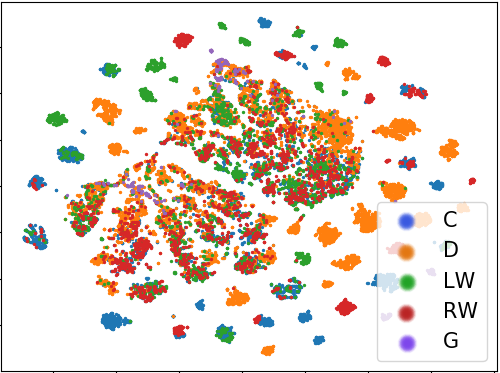
\includegraphics[width=0.3\columnwidth]{./figures/embedding-visualization-position.png} }}%
    {{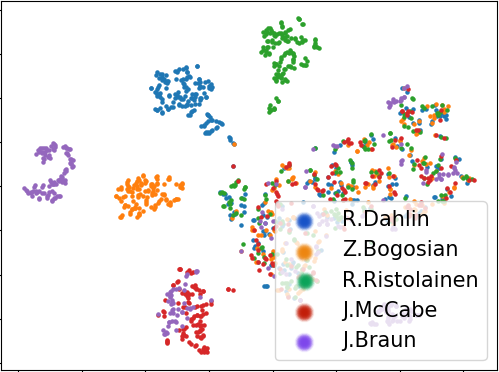
\includegraphics[width=0.3\columnwidth]{figures/embedding-visualization-defence.png} }}%
    {{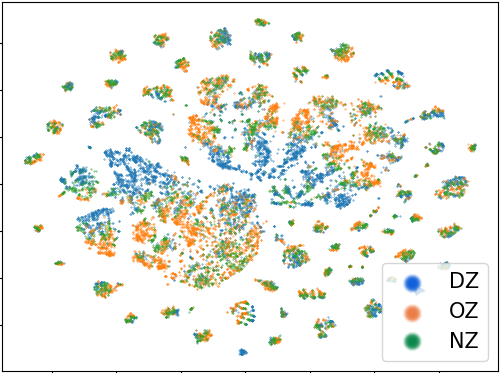
\includegraphics[width=0.3\columnwidth]{./figures/embedding-visualization-zone.png} }}%
    {{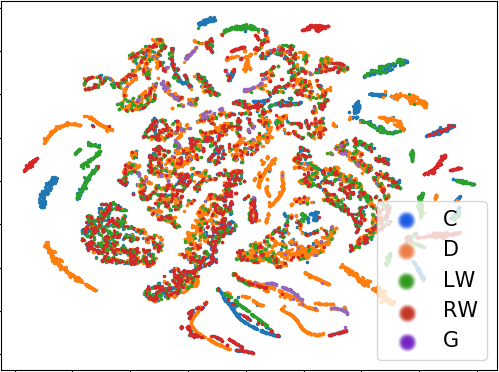
\includegraphics[width=0.3\columnwidth]{./figures/embedding-visualization-caernn-position.png} }}%
    {{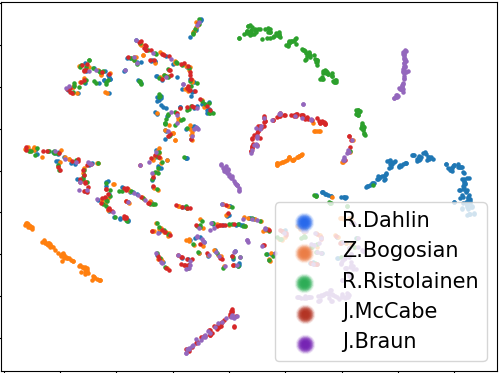
\includegraphics[width=0.3\columnwidth]{figures/embedding-visualization-caernn-defence.png} }}%
    {{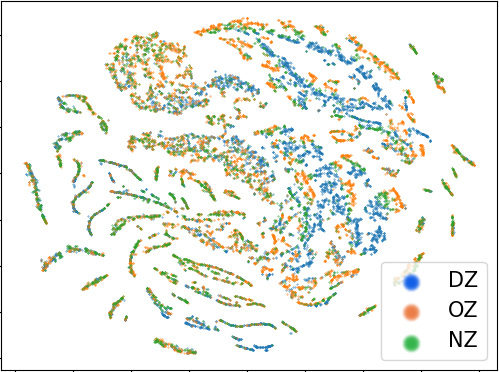
\includegraphics[width=0.3\columnwidth]{./figures/embedding-visualization-caernn-zone.png} }}%
    \caption{Embedding visualization. Each data point corresponds to a player embedding conditioning on the game context at the current %event (or 
    time step $t$.  
    The player embeddings are labelled 1) player positions (on the {\it left} column, including Center (C), Defense (D), Left-Wing (LW) and Right-Wing (RW) and Goalie (G)) 2) 5 selected defence men (on the {\it middle} column) and 3) player locations (on the {\it right} column, including Defence Zone (DZ), Neutral Zone (NZ) and Offensive Zone (OZ)). The embeddings are computed by \system ({\it top plots}) and CAERNN ({\it bottom plots}) respectively.} 
    \label{fig:embedding-visualization}%
\end{figure}

\subsection{Predictive Performance On Application Tasks}
~\label{subsec:downstream-applications}
We validate our \system model by feeding the generated embeddings to other application models and studying their influence on the model performance in practical application tasks.

{\bf Expected Goals Estimation:} We validate the player embeddings for the practical 
task of estimating the Expected Goal (XG). 
An XG metric is a shot quality model that weights each {\it shot} by its chance of leading to a goal~\cite{Macdonald2012}.
We incorporate $\latentvariables_{t}$ from the learned player representations into XG prediction. 
At time $t$, we input $\state_{t},shot_{t},\latentvariables_{t}$ to the application model $\zeta$ (implemented as a RNN), which is trained to output $p(\it{goal}_{t+1}|\state_{t},\it{shot}_t,\latentvariables_{t})$: the probability that a goal is scored after the player $\player_{t}$ makes the shot.
% and 0 otherwise.
Our dataset provides ground-truth labels for whether a given shot led to a goal. 
% The model is trained with the game context for action shot in our NHL dataset and we supervise the training by whether the shot will lead to a goal in real games. 
Since only a few shot attempts lead to a goal ($<$3.9\%), the training data is highly imbalanced.
% , which will encourage the model to label all the shots as 0, in order to %improve the overall prediction accuracy. 
We %, therefore, 
employ a resampling method~\cite{good2006resampling} so that successful and failed shots %(e.g. blocked or missed) 
 occur equally often during training.

\begin{table}[htbp]
    \centering
% \addtolength{\tabcolsep}{-1.5pt} 
    \caption{Expected goal results 
    % Results for predicting the Expected Goal 
    applying different player embeddings. 
    % The evaluation metrics include Precision (P), Recall (R) and F1-score.
    }
    \label{table:exp-eg}
    \resizebox{0.8\textwidth}{!}{
    \begin{tabular}{c|cccc}
        \toprule
        \multirow{2}{*}{\begin{tabular}[c]{@{}c@{}}Player Embedding\\ Method\end{tabular}} & \multicolumn{4}{c}{Performance} \\ \cline{2-5}
        & Precision & Recall & F1-score & AUC \\ \hline\hline
        % $\emptyset$ 
        N/A &  0.12  $\pm$  1.75E-4 & 0.79  $\pm$  9.46E-4 & 0.21  $\pm$  4.26E-4 &  0.86  $\pm$  3.56E-4\\
        Pids  & 0.09  $\pm$  1.62E-4 & 0.62  $\pm$  2.52E-3 & 0.15  $\pm$  4.20E-4 & 0.70  $\pm$  1.25E-3\\
        DE  & 0.30  $\pm$  1.26E-4 & 0.92  $\pm$  4.21E-4 & 0.45  $\pm$  1.87E-4 & 0.96  $\pm$  1.86E-5\\
        CVAE & 0.33  $\pm$  5.33E-5 & 0.95  $\pm$  8.72E-5 & 0.49  $\pm$  8.29E-5  & 0.96  $\pm$  1.13E-6\\
        MA-BE & 0.35  $\pm$  1.44E-4 & 0.91  $\pm$  2.30E-4 & 0.50  $\pm$  1.56E-4 & {\bf 0.97}  $\pm$  1.46E-6\\
        CAERNN & 0.29  $\pm$  1.05E-4 & 0.96  $\pm$  1.56E-4 & 0.44  $\pm$  1.65E-4 & 0.95  $\pm$  1.27E-5\\
        CVRNN  & {\bf 0.40}  $\pm$  4.75E-4 & 0.84  $\pm$  1.81E-4 & 0.54  $\pm$  2.97E-4 & 0.96  $\pm$  4.07E-6\\ 
        \system & 0.37  $\pm$  2.01E-4 & {\bf 0.98}  $\pm$  1.32E-4 & {\bf 0.54}  $\pm$  8.14E-5 & 0.96  $\pm$  2.23E-6 \\\bottomrule
    \end{tabular}
    }
\end{table}

Using the most likely label as the predicted class, Table~\ref{table:exp-eg} shows the accuracy results on the testing set. 
Without including any player information (N/A), predictions have very limited precision, because the model does not have access to player information that would allow it to distinguish above-average from below-average shooters.
% On this dataset, achieving high precision is a difficult challenge. 
Adding the pids to the input does provide this information, but the prediction model fails to take advantage of it. This shows that player information is difficult to utilize from a sparse one-hot representation.
%label conveys only limited player information. 
Applying the embeddings from a player encoder (e.g. DE and CVAE)  improves both precision and recall, but the improvement is limited by the lack of game history information.
Among the recurrent models, \system achieves the highest recall and F1-score with good precision. This is because shooting strength correlates with the learned player types, which are most accurately represented by our model.


{\bf Score Difference Prediction:}\label{subsec:score-diff}
Dynamic Score Difference Prediction (DSDP) is a recently introduced task~\cite{ganguly2018problem}: 
%that requires to 
predict the final score difference $\scorediff(T)$ under a game context ($\state_{t},\action_{t}$) where $t$ runs from 0 to $T$ (game ends). 
In preliminary experiments, we observed that traditional supervised learning methods suffer a large training variance (especially early in the game when many outcomes are equally likely).
%, and thus fail to converge. 
To exploit the temporal dependencies between score differences at successive times, we apply reinforcement learning; specifically the temporal difference method Sarsa prediction~\cite{sutton2018reinforcement}. Sarsa learns a Q-function for a generic home/away team to estimate the expected cumulative goal scoring: $Q_{\team}(\state_{t},\action_{t})= \expect(\sum_{\tau=t}^{T}\goal_{\team,\tau})$ where $\team=\home/\away$ and $\egoal_{\team}$=1 if the team scores at $t$ and 0 otherwise. From Q-functions, the Predicted Score Difference (PSD) at $t$ is given by % \begin{equation}
$\it{PSD}(t)= Q_{\home}(\cdot)-Q_{\away}(\cdot) + \scorediff(t)$.
% \end{equation}
Our {\em application model $\zeta$} is a DRQNN~\cite{littlestone} that computes the Q-functions. The inputs are state $\state_{t}$, action $\action_{t}$ and the embedding $\latentvariables_{t}$ for the acting player $\player_{t}$. 
For each testing game $m$ and time $t$, the absolute error is given by  $ |\it{PSD}(t_m)-\scorediff(T_m)|$. 
For each game time $t$, Figure~\ref{fig:temporal-diff} plots the mean and the variance of the absolute error over all testing games $m=1,\ldots,M$. 
% (, where $m\in[0, M]$ and $M$ denotes the number of testing games), at each time step $t$. 
The plot shows a larger difference between real and predicted SDs at the beginning of a game, but the mean and variance of the difference become smaller towards the game end. Among the evaluated embedding methods, our {\em \system (the black line) manages to generate the player representations that lead to the most accurate predictions.} We also find that the accuracy advantage is strongest towards the early game, especially compared to the N/A and pids. This indicates that an informative player representation significantly alleviates the difficulty of predicting multiple outcomes early in the  game. 
Averaging over game times $t$ defines the game prediction error for each tested game $m$. Table~\ref{table:avg-diff} reports the mean and standard deviation for the game prediction error.
% , We also report the average Mean Absolute Error (MAE) over all game times in Table~\ref{table:avg-diff}. 
The \system embeddings yield the lowest Mean Absolute Error (MAE).

\begin{table}[htbp]
\begin{minipage}[t]{.7\textwidth}
    \centering
    \subfloat{{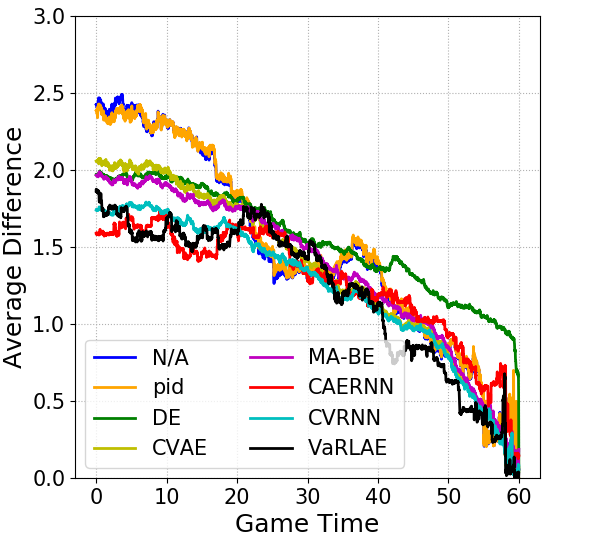
\includegraphics[width=0.45\columnwidth]{./figures/temporal-absolute-difference-plot.png}}}%
    % \quad
    \subfloat{{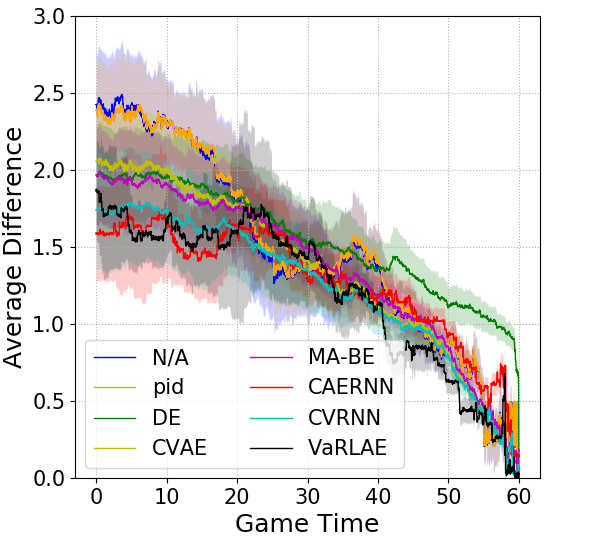
\includegraphics[width=0.45\columnwidth]{./figures/temporal-absolute-difference-shadow-plot.png} }}%
    \captionsetup{width=.95\linewidth}
    \captionof{figure}{Temporal illustrations of the absolute error between predicted score differences and final score differences.
    % applying different embeddings. 
    The plots report mean (left) and mean$\pm$variance of the differences (right). Appendix shows the separated plots for each method.}
    \label{fig:temporal-diff}
\end{minipage}%
\begin{minipage}[t]{.3\textwidth}
    \caption{The test set game prediction error between predicted and final score differences for the entire game.}
    \label{table:avg-diff}
    \resizebox{0.9\textwidth}{!}{
    \begin{tabular}{c|c}
    \toprule
    Method  &  MAE \\\hline\hline
    N/A & 1.55 $\pm$ 0.35 \\
    Pid & 1.56 $\pm$ 0.32 \\
    DE & 1.48 $\pm$ 0.24  \\ 
    CVAE & 1.49 $\pm$ 0.29 \\
    MA-BE & 1.45 $\pm$ 0.25 \\
    CAERNN & 1.31 $\pm$ 0.23 \\
    CVRNN & 1.32 $\pm$ 0.27 \\
    \system & {\bf 1.28} $\pm$ 0.29\\
    \bottomrule
    \end{tabular}
    }
\end{minipage}
\end{table}

\section{Conclusion}
Capturing what team sports players have in common and how they differ is one of the main concerns of sports analytics. This work introduces a {\it player representation via player generation} framework that learns deep contextualized representations for ice hockey players. We described a \system model for sports data, based on a Markov Game model representation. The ELBo loss (Equation~(\ref{eq:elbo})) induces a shrinkage effect such that similar players are mapped to similar representations in similar match contexts. We validate the player representation on two downstream applications that are important in sports analytics: predicting expected goals and final match score differences. While our evaluation focuses on ice hockey, our approach is general and can be applied to other team sports, or indeed any strategic setting that can be modelled as a Markov game with many participants. A direction of future work is to combine player representations with modelling player interactions. Another is learning representations for different lineups, given a dataset with  full observations of on-court players.
% \footnote{\textcolor{red}{OS:We could drop future work if space is tight.}}

\section{Broader Impact}
We expect the main impact outside of the machine learning community to be in professional sports. As an entertainment industry, professional sports increases the quality of life for many people. With respect to the broad challenges of our society (polarization, inequality, bias), entertainment is in our view neutral. %Our work provides an objective data-driven method for understanding what is special about individual players. 
The main stakeholders impacted will be sports teams, managers, and athletes.  For sports stakeholders, we expect mainly positive and some negative outcomes. 

{\bf Positive Outcomes.} Our work significantly enhances the reliability of the machine learning algorithm on modeling complex sport dynamics. This allows teams, coaches, and fans to better understand a player's style, influence, and contributions. The result will be better and even more enjoyable sports. 
For sports stakeholders, the main positive outcome will be that coaches can deploy players more effectively, which will help them display and improve their considerable skills. This will create winners and losers among the players, but on the whole, a A data-driven approach will increase fairness and objectivity in player performance ranking, while decreasing bias. Bias towards underrepresented groups is known to hurt the perception and career chances of underrepresented groups, such as indigenous ice hockey players; Fred Sasakamoose is a prominent example.  

{\bf Negative Outcomes.} Putting players' performance and contribution under intense study may lead to more performance pressure on the professional players. We believe that for most players this Taylorist pressure~\cite{bib:taylorism} is outweighed by the guidance for how to improve both their play and their market value. To apply our model, sports team should invest in technical analytic resources, which might not be affordable for small clubs. It potentially increases the inequality between top-ranked teams and lower-ranked teams. To help level the analytics playing field, we have placed our code in the public domain at github\footnote{\url{https://github.com/Guiliang/player-embedding-ice-hockey}}.

% sports analytics has played an important role in professional sport. The traditional sports analytic is very empirical, basing on the manually collected box scores (player statistics) and human experience. With the advancement of high-frequency optical tracking and object detection systems, more and larger event stream datasets for sports matches have become available. These data provide an increasing opportunity for developing data-driven machine learning models, which extends the recent progress on artificial intelligence to sports analytics and significantly improve the performance of many previous study sports analytic task.
% However, the application of machine learning in sports analytics is still new and largely unexplored. Our work is a fundamental step that allows studying how the specialty of different players influences action success and game outcomes.

% {\bf Positive Outcomes.} 1) Our work significantly enhances the reliability of the machine learning algorithm on modeling complex sport dynamics. 2) Our work allows teams and fans to better understand a player's influence and contributions. It can influence a team's decision on trading or recruiting players. 3) Our work can attract the academy's attention to the field of sports analytic.

% \paragraph{Negative Outcomes.} 
% The players' performance and contribution are under intense study, which indicates more pressure to the professional players.

% \textcolor{blue}{Authors are required to include a statement of the ethical aspects and future societal consequences. Authors should take care to discuss both positive and negative outcomes.
% }

\begin{ack} This project was supported by a Strategic Project Grant from the Natural Sciences and Engineering Research Council of Canada. We are grateful for helpful comments from Jesse Davis, Tim Swartz, and the reviewers and participants in the 2019 AAAI Team Sports workshop. Our computations were facilitated by a GPU donation from NVIDIA.

% Use unnumbered first level headings for the acknowledgments. All acknowledgments go at the end of the paper before the list of references. Moreover, you are required to declare funding (financial activities supporting the submitted work) and competing interests (related financial activities outside the submitted work). More information about this disclosure can be found at: \url{https://neurips.cc/Conferences/2020/PaperInformation/FundingDisclosure}.

% Funding in direct support of this work: NSF grant XXX, GPUs donated by YYY, scholarship by Company ZZZ.

% Additional revenues related to this work: Sabbatical at Company Y; Part time employment with Company Z; Honorarium for lectures by Charity X; Honorarium as Member of the Advisory Board of Startup C; Travel support by Foundation A; hardware donations by Company B.

% Do {\bf not} include this section in the anonymized submission, only in the final paper. You can use the \texttt{ack} environment provided in the style file to autmoatically hide this section in the anonymized submission.
\end{ack}

\bibliographystyle{unsrt}
\bibliography{master}
\end{document}